%
% File naacl2019.tex
%
%% Based on the style files for ACL 2018 and NAACL 2018, which were
%% Based on the style files for ACL-2015, with some improvements
%%  taken from the NAACL-2016 style
%% Based on the style files for ACL-2014, which were, in turn,
%% based on ACL-2013, ACL-2012, ACL-2011, ACL-2010, ACL-IJCNLP-2009,
%% EACL-2009, IJCNLP-2008...
%% Based on the style files for EACL 2006 by 
%%e.agirre@ehu.es or Sergi.Balari@uab.es
%% and that of ACL 08 by Joakim Nivre and Noah Smith

\documentclass[11pt,a4paper]{article}
\usepackage[hyperref]{naaclhlt2019}
\usepackage{times}
\usepackage{graphicx}
\usepackage{latexsym}
\usepackage{amsmath}
\usepackage{bm}

\newcommand{\rdep}[1]{\ $\xrightarrow{\text{\tiny #1}}$\ }
\newcommand{\ahcomment}[1]{\textcolor{blue}{[#1 -AH]}}

\usepackage{url}

%\aclfinalcopy % Uncomment this line for the final submission
%\def\aclpaperid{***} %  Enter the acl Paper ID here

%\setlength\titlebox{5cm}
% You can expand the titlebox if you need extra space
% to show all the authors. Please do not make the titlebox
% smaller than 5cm (the original size); we will check this
% in the camera-ready version and ask you to change it back.

\hypersetup{draft} % THIS IS NEEDED TO GET IT TO COMPILE. Does not like the tables. AH 11/27

\newcommand\BibTeX{B{\sc ib}\TeX}

\DeclareMathOperator*{\argmaxA}{arg\,max} % Jan Hlavacek

\title{Extractive sentence compression under lexical and length constraints}

\author{First Author \\
  Affiliation / Address line 1 \\
  Affiliation / Address line 2 \\
  Affiliation / Address line 3 \\
  {\tt email@domain} \\\And
  Second Author \\
  Affiliation / Address line 1 \\
  Affiliation / Address line 2 \\
  Affiliation / Address line 3 \\
  {\tt email@domain} \\}

\date{}

\begin{document}
\maketitle

\begin{abstract}
Traditional approaches to extractive sentence compression seek to reduce the length of a sentence, while retaining the most ``important'' information from the source. But query-focused applications such as document search engines or exploratory search interfaces place additional lexical and length requirements on compression systems. This study introduces a new, linguistically-informed compression method which can accommodate such requirements.  Our method is more computationally efficient than classical ILP-based approaches, and more accurately reconstructs known-good shortenings.
\end{abstract}

\section{General comment}
Nobody cares about Rookie. Make the argument for open source search engines. 

\ahcomment{TODO: Brendan's email}

\section{Unknowns}

\ahcomment{How will we deal with semantics? Brendan email about subsective adjectives ellie pavlik work. Right now we just use the gold data for this I guess. Future work?}

\ahcomment{How to use data from Brian, if at all. It uses dep type info + LM info + worker info. We use dep type info already. Can we use LM info?}

\section{Introduction}

Traditional study of extractive sentence compression seeks to create short, readable compressions which retain the most ``important'' information from source sentences. But query-focused and user-facing applications impose additional requirements on the output of a compression system. Compressions must be short enough to be shown in a user interface; and often must contain a user's query term. An example of such a compression is shown in Figure \ref{f:qf}.

This study examines the compression problem with length and lexical constraints: shortened sentences must meet a given character budget, and must include particular words. While older compression methods based on integer linear programming could trivially accommodate such restrictions, recent work has focused on neural network techniques \cite{filippova2015sentence} which do not give practitioners such control. This makes existing neural methods unsuitable for search engines \cite{hearst2009search}, concept map browsers \cite{falke2017graphdocexplore} and new forms of exploratory textual interfaces \cite{marchionini2006exploratory}, where length and lexical constraints are paramount. 

\begin{figure}[htb!]
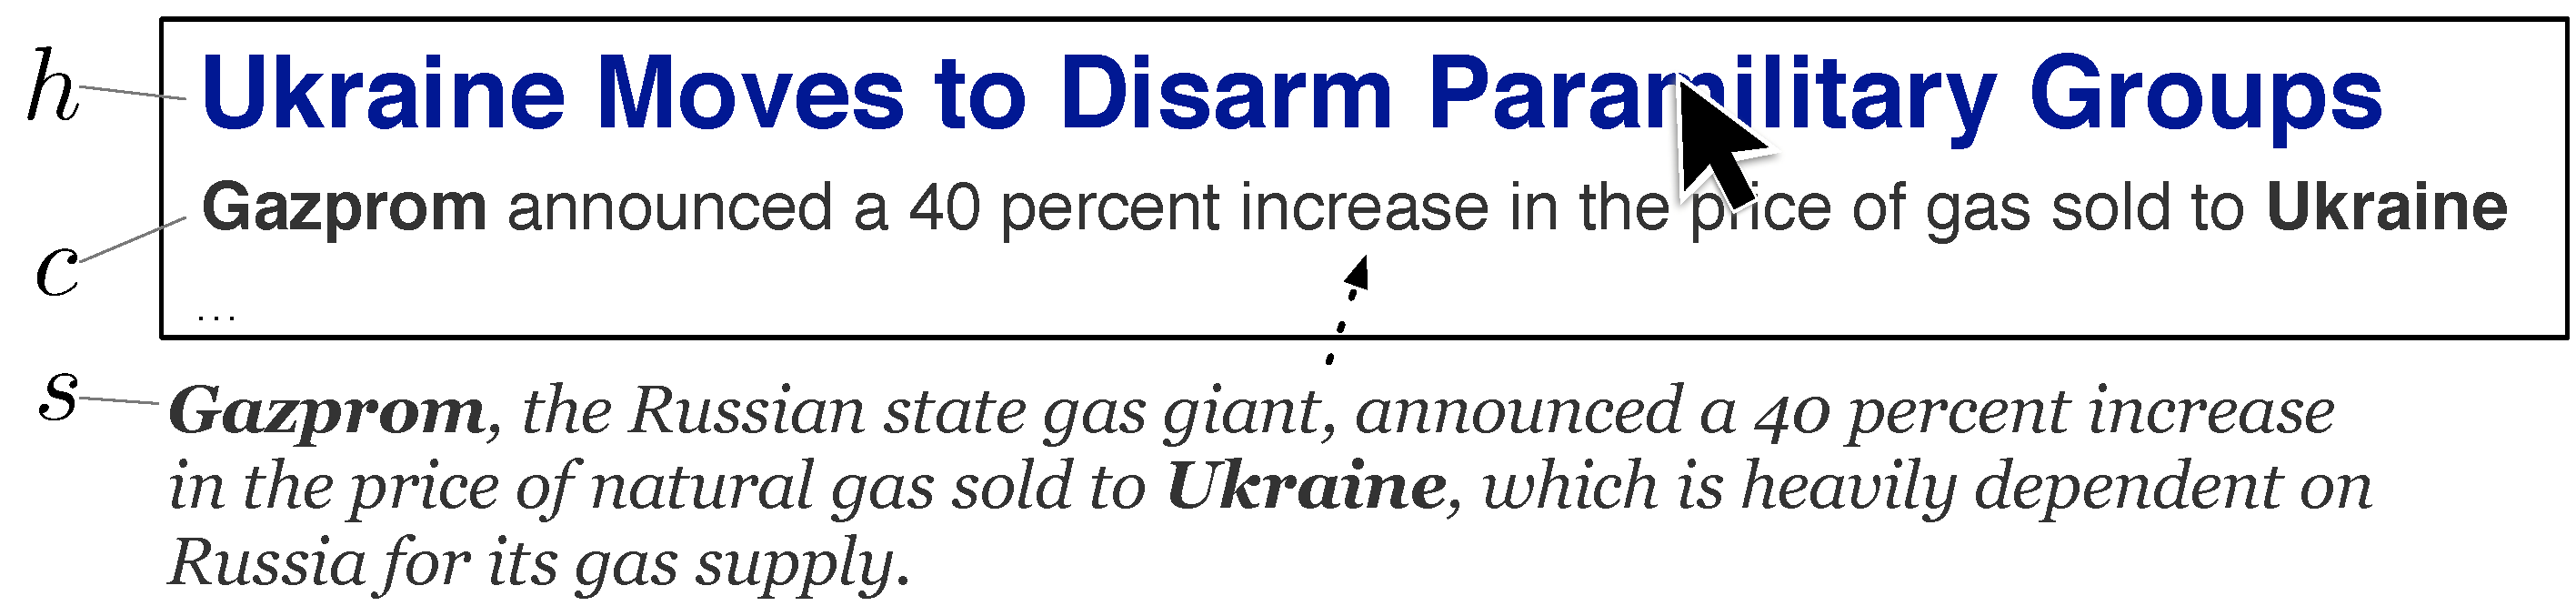
\includegraphics[width=9cm]{qf.pdf}
\caption{Search interfaces often require compressions with length and lexical constraints. In this case, the user has queried for ``Pemex contracts"; a system returns a related link and a short compression which contains the query terms}
\label{f:qf}
\end{figure}


Therefore, in this work:

\begin{itemize}
\item{We present a new, linguistically-informed method for compressing sentences, which leverages the large corpora used to train neural networks, while also accommodating lexical and length constraints.}
\item{Compare our transition-based technique to traditional ILP-based methods, which also give a user such control.}
\item{We analyze the computational costs of each technique, as well as the nature of the constrained compression problem itself}
\end{itemize}


\section{Compression and constraints}

This work discusses contrasts traditional ILP-based compression with our novel transition-based technique. We also briefly discuss compression with LSTM taggers, which do not accommodate length or lexical requirements.

\begin{table*}[htb!]
\begin{tabular}{cccc}
\textbf{Approach} & \textbf{Worst-case complexity} & \textbf{Constrained} & \textbf{Allows supervision} \\ \hline
LSTM taggers      & linear              & no     &    yes      \\   
linear programming              & exponential         & yes    &    yes   \\
transition-based (this work)       & quadratic*           & yes    &      yes   \\
\end{tabular}
\caption{\ahcomment{TODO}}
\end{table*}

\subsection{Constrained compression with ILPs}

One common approach for shortening sentences formulates compression as an integer linear programming (ILP) task. ILP-based methods assign binary variables to each token in a sentence \cite{clarke2008global} or subtree in a dependency parse \cite{filippova2008dependency}. These variables indicate if the corresponding component included in a compression. Each such sentence component is also assigned a local weight, indicating its worthiness for inclusion in a shortened sentence. Local weights are either learned with structured perceptron techniques \cite{filippova2013overcoming}, or inferred from corpus statistics \cite{filippova2008dependency}, word importance scores and language models \cite{clarke2008global}.

ILP methods represent the overall quality of a compression by summing the local weights of sentence components to compute a global objective score.  The problem of identifying the best possible solution to an integer programming compression objective is exponential in the number of tokens or number of subtrees in the input, as each binary variable may be set to zero or one. Researchers use off-the-shelf ILP solvers to identify the highest-scoring compression, from among the exponential possible configurations of binary variables.

This integer linear programming approach also easily accommodates constrained compression. When performing ILP-based compression, researchers will customarily add constraint terms to the ILP objective in order to preserve the meaning of a sentence (e.g. don't remove negations), or to ensure that output forms a valid tree (e.g. each subtree must have a parent vertex).

For these methods, adding additional length or lexical requirements is trivial: practitioners must specify that optimal solutions must be shorter than some character budget and must specify that binary variables marking inclusion of particular words must be set to 1. 

\subsection{Transition-based constrained compression}

In this work, we present an alternative method for shortening sentences under lexical and length constraints. Our transition-based technique compresses a sentence over $N$ time steps, by adding and removing $N$ different subtrees from a dependency parse, one after another. This method recalls early solutions to the compression problem \cite{Jing2000SentenceRF,Knight2000StatisticsBasedS}, which also shortened sentences by executing grammatically-motivated operations on syntactic representations of trees. \ahcomment{argue for coverage w/ F and A at some point} We present the formal details in \S\ref{s:system}.

Like ILP-based methods, transition-based approaches can easily accommodate lexical and length restrictions. At a high-level, such methods need to add subtrees which contain query terms and remove subtrees which do not contain subtrees, until identifying a compression which satisfies the length constraints. In this work, we show that transition-based methods incur much smaller computational costs than integer programming techniques, while achieving higher token-level F1 scores than ILP-based compression.

\subsection{Unconstrained compression with LSTMs}

We contrast transition-based compression and integer programming approaches with LSTM taggers for the compression task \cite{filippova2015sentence}. Such taggers achieve state-of-the-art scores on extractive sentence compression, using sequence-to-sequence models that label tokens with a 1 or a 0 indicating if the token should be included in a summary. This approach achieves state-of-the art performance, and is linear in the token length of a the input sequence. However, at this time, LSTM taggers are unsuitable for query-focused applications because such methods cannot enforce lexical or length requirements. This limitation might be examined in future research.

\section{Transition-based sentence compression}\label{s:system}

In this work, we define a neural, transition-based sentence compression system, inspired by recent successes in neural dependency parsing \cite{D14-1082}. Let ${(V_s,E_s)}$ denote the original, unchanging dependency parse of a sentence. At each timestep during compression, our system has a state ${(V_c,E_c)}$, which is some subgraph of ${(V_s,E_s)}$. The compression ${(V_c,E_c)}$ may or may not be fully-connected. 

We define two operations which modify the state. The operation \textsc{Prune}($v_c$), removes the subtree rooted at $v \in V_c$ from ${(V_c,E_c)}$. The operation \textsc{Insert}($v_s$), copies the subtree rooted at $v \in V_s$ in the original sentence and adds it to the compression ${(V_c,E_c)}$. After executing a sequence of $\textsc{Prune}$ and $\textsc{Insert}$ operations, all tokens in ${(V_c,E_c)}$ are linearized in their original order to return a shortened sentence. We initialize the state with an empty subgraph. 

We defined $\textsc{Prune}$ and $\textsc{Insert}$ via empirical experiment: we found that for all compressions in a large, standard  corpus \cite{filippova2013overcoming} there exists an oracle path of at most $|V_s|$ $\textsc{Prune}$ and $\textsc{Insert}$ operations which can fully reconstruct the shortened sentence. 

\begin{figure*}[htb!]
\centering
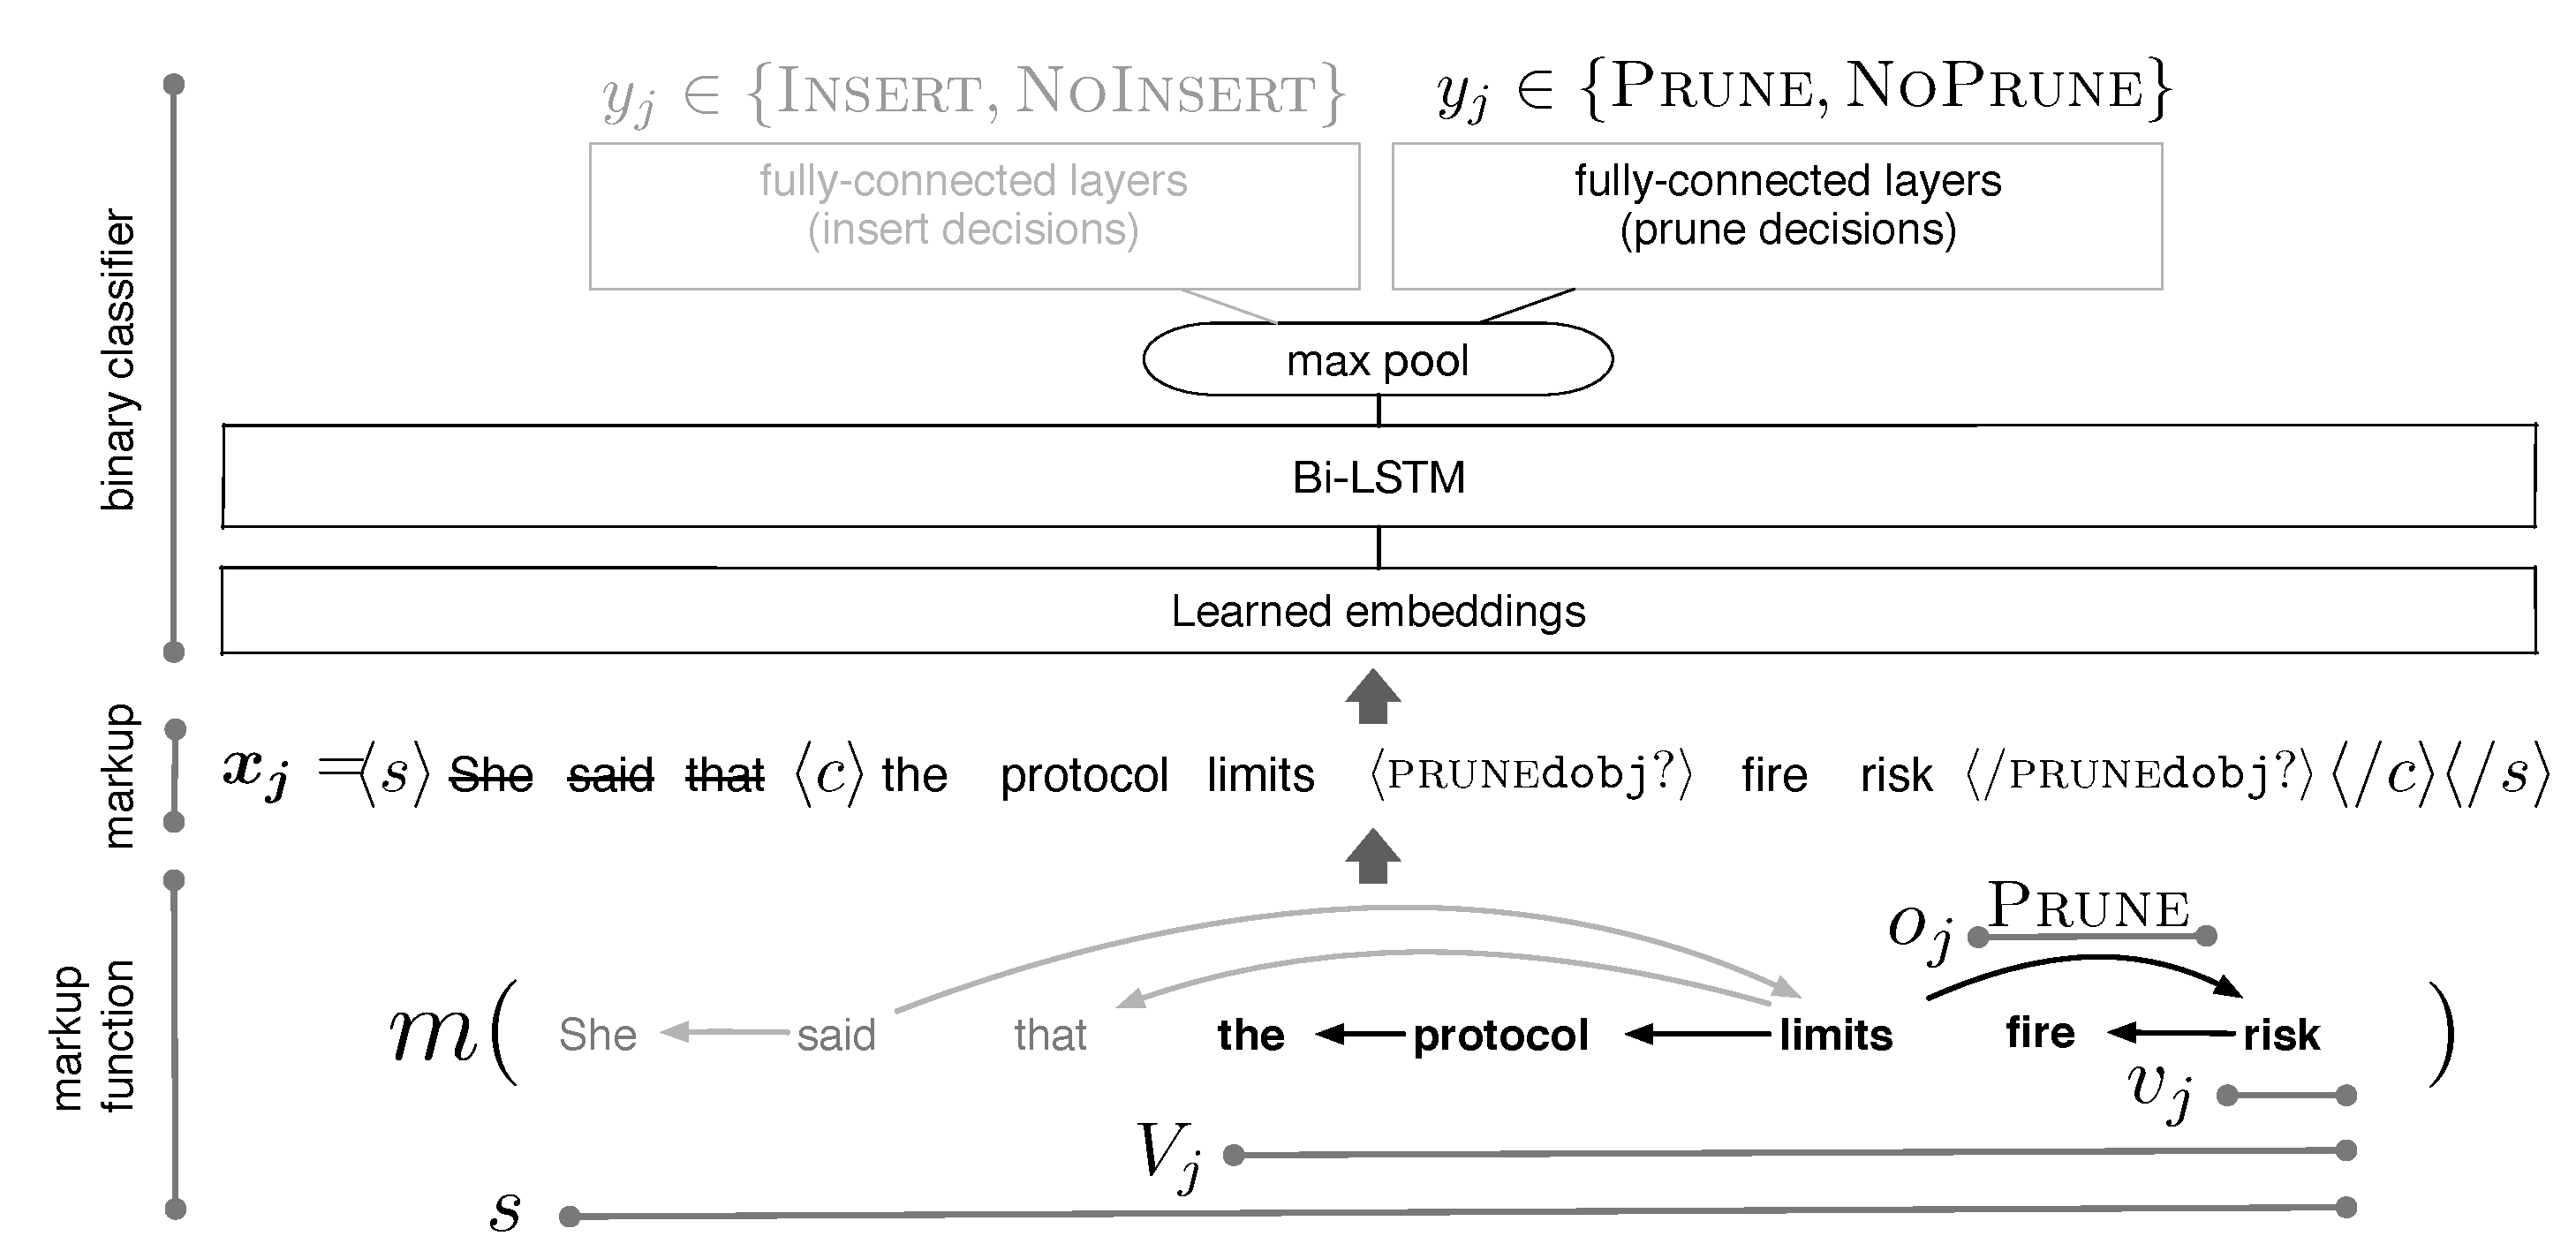
\includegraphics[width=.75\textwidth]{example.pdf}
\caption{Our LSTM classifier predicts the oracle operation given the current state $(V_c, E_c)$, which is a subgraph of the original sentence (top). The input to the classifier is all tokens in $V_c$,  linearized in their original order between added SOS and EOS tags which indicate the start and end of the sequence. We also add insert marker symbols with dependency type information denoting the start and end of the sequence of tokens which would be modified by the \textsc{Prune} or \textsc{Insert} operation. In this example, the subsequence ``in limiting risk'' would be pruned by removing a subtree governed by an \rdep{advcl} relation. For \textsc{Insert} operations, we include proposed tokens between marker symbols.}
\label{f:example}
\end{figure*}

Like \citet{D14-1082}, we use a large corpus to identify a series of oracle operations which returns gold standard output. In our case, we assign an oracle operation to each $v \in V_s$, by walking the dependency parse of an original sentence breadth-first, and identifying which operation on $v$ is consistent with the gold-standard compression. For instance, if some vertex $v$ and all of its children are not present in the gold compression, but are present in ${(V_c,E_c)}$ at a given timestep, then we say that the oracle operation for $v$ is \textsc{Prune}. Similarly, if $v$ is present in the gold compression, but is not present in ${(V_c,E_c)}$ at a given timestep, we say that the oracle operation for $v$ is \textsc{Insert}. For roughly two-thirds of vertexes in the breath-first walk, the oracle does not execute a $\textsc{Prune}$ or $\textsc{Insert}$ operation. In these cases, we say that the oracle executes a $\textsc{Nop}$, which leaves ${(V_c,E_c)}$ unmodified. 

In our transition-based compressor, only some operations are valid for some configurations of the state. If some vertex $v \in V_s$ is also included in the compression, then we say that $\textsc{Insert}(v)$ is not valid as $v$ is already present in the compression. Similarly, if some vertex $v^{\prime} \notin V_c$ is not included in the compression, then we say that $\textsc{Prune}(v^{\prime})$ is not valid as $v^{\prime}$ cannot be pruned.

All $v \in V_s$ are either in $V_c$ or not in $V_c$. Therefore, for any given vertex--state pair, either the operation \textsc{Prune} is valid or the operation \textsc{Insert} is valid. We can therefore distinguish between two subtypes of $\textsc{Nop}$ operation. If the oracle does not prune a given subtree, we say that the oracle executes $\textsc{Nop}_P$. If the oracle does not insert a given subtree, we say that the oracle executes $\textsc{Nop}_I$. This distinction is helpful during modeling because the state--vertex pairs which correspond to $\textsc{Nop}_I$ are very different to the pairs which correspond to $\textsc{Nop}_P$.

\subsection{Modeling}\label{s:modeling}

We use a large, standard compression corpus \cite{filippova2013overcoming} to train a model of transition-based compression. Following \citet{D14-1082}, we interpret the collection of oracle paths (\S\ref{s:system}) for all sentences in the corpus as a set of tuples: ${((V_c,E_c)_j, y_j)}$, where $(V_c,E_c)_j$ is the state of the system at step $j$ along the oracle path and $y_j \in  \{ \textsc{Prune}(v_c), \textsc{Insert}(v_s), \textsc{Nop}_P, \textsc{Nop}_I \}$ is the oracle operation at step $j$. We then train an ordinary LSTM classifier to predict the oracle operation, given the state. 

\ahcomment{this is a bit weird; easier/less weird than 2 models?} Because only a \textsc{Prune} or \textsc{Insert} operation is valid for a given vertex--state pair, it is possible to interpret our 4-way classifier as two 2-way classifiers. The added prune and extract symbols added to the input sequence provide very strong hints about which operation subset of operations might be chosen for a given vertex. 

During training, we look up each token in the sequence in an embeddings matrix and pass these embeddings to a Bi-LSTM. Following recent work on LSTM classification for sentence-level tasks \cite{D17-1070}, we use a max pooling layer to encode a variable-length sequence into a fixed-length vector, which we pass through a sigmoid and then softmax layer to predict the oracle operation. We train using cross entropy loss, weighting training examples in proportion to their prevalence in the dataset. 


\ahcomment{details of weighting}

\ahcomment{comment on projectivity}

\ahcomment{details of optimizer}

\ahcomment{details of stopping criteria}

\ahcomment{details of embeddings}

\ahcomment{loss function}

\ahcomment{do you update embeddings?}

\ahcomment{tuning}

\subsection{Markup function}

We define a markup function, $m$ which takes the state of the compression system $(V, v|B)$ as input, and returns a sequence of symbols $\bm{x}$, called \textbf{the markup}. Recall that $V$ is a set of vertexes, and $v$ is a single vertex in the first position of $B$, the buffer (\S\ref{s:system}). Intuitively, the markup ``shows'' the LSTM what the sentence would ``look'' like if $T(v)$ were to be inserted into or pruned from the sentence. 

More formally, we again use $T(v)$ to denote all vertexes in the subtree governed by $v$ in $s$. We then define $V_L \subseteq V$
to be is all tokens in $V$ which occur to the left of  $T(v)$ in $s$; and define $V_R \subseteq V$ to be all tokens in $V$ which fall to the right of $T(v)$ in $s$. We also define a linearization function, $\ell(  \{v_1, v_2 ... v_n \}, s)$, which returns all vertexes in some set $\{v_1, v_2 ... v_n \}$, linearized in their order in $s$.\footnote{$\ell$ is needed because sets do not have order} 

The markup is the sequence, [SOS, $\ell(V_L)$, StartTag, $\ell(T(v))$, EndTag, $\ell(V_R)$, EOS], where SOS and EOS are out of vocabulary symbols denoting the start and end of the sequence. The StartTag included in the markup is an out of vocabulary symbol formed by concatenating markers which indicate (1) the dependency type governing $T(v)$ (2) the type of operation (i.e \textsc{Prune} or \textsc{Insert}) and (3) the position of the StartTag to the left of $\ell(T(v))$. If there are $D$ dependency types there are $D \times 2$ possible StartTag symbols. The EndTag is identical, except that the final marker indicates that the EndTag occurs to the right of $\ell(T(v))$. 

Figure \ref{f:example} shows an example. Such marker symbols allow us to encode some aspects of syntax trees using a standard sequence model \cite{Vinyals2015GrammarAA,Aharoni2017TowardsSN}, without the added complexities of explicitly modeling nested structures \cite{Tai2015ImprovedSR,Dyer2016RecurrentNN}. 

We note that it is only possible to $\textsc{Prune}$ $T(v)$ if $v \in V$, and only possible to \textsc{Insert} $T(v)$ if $v \notin V$. Therefore, the marker indicating the type of the operation included in the StartTag and EndTag is fully determined by the inputs to $m$. 

\section{Experiment: Automatic Evaluation of Constrained Compression}

We use a large, standard dataset of sentence--compression pairs from \citet{filippova2013overcoming} to both train and evaluate different approaches to length and lexically constrained compression. Using the dataset in this manner requires reinterpreting gold standard data, which does not specify either a query or length constraint. After re-tokenizing, parsing and tagging NER spans with Stanford CoreNLP 3.8.0 \cite{corenlp}, we define all NER tokens\footnote{We use a standard 3-class definition of NER; for our purposes, entities are people, locations or organizations.} which lie within the gold compression as the query, $q$. Formally, $q$ is a list of tokens. We also define the character length of the gold-standard compression as the character budget, $b$. This interpretation allows us to redefine the corpus of $(s,c)$ pairs as a corpus of 4-tuples $(q,s,b,c)$, where $q$ is the query, $s$ is the original sentence, $b$ is the character budget and $c$ is some readable compression which satisfies the length and lexical constraints.  \ahcomment{Note: these Q and r are going to be well-behaved! I.e. there is usually a good compression here. Should be revisited.}

We then use token-level F1, to measure how well an ILP-based method (\S\ref{s:ilp}) and a transition-based method (\S\ref{s:transition}) method can reconstruct each known-good compression $c$, given $q,s$ and $b$. Token-level F1 is the standard automatic evaluation metric for the sentence compression task. We describe each method in the following sections.

\ahcomment{human eval?}
    
\begin{table}[htb!]
\begin{tabular}{ll}
\centering
Approach & F1  \\ \hline
Human acceptability supervision \ahcomment{????}        &  X        \\
F and A (2013)    & .79           \\
C and L (2008)  \ahcomment{????}  & X      \\
\textbf{Transition-based (this work)} &  \textbf{.86}    \\   
\end{tabular}
\end{table}

\ahcomment{todo p-values}


\subsection{Implementation: transition-based compression}\label{s:transition}

Our model of transition-based sentence compression (\S\ref{s:modeling}) predicts the oracle operation $y$, given the state $(V_c, E_c)$. There are many possible ways to use $p(y|(V_c, E_c)$ in a query-focused and length-constrained compression system. We use a simple \textbf{iterative deletion} technique: at each step $j$ we \textsc{Prune} the subtree rooted at 

$$\argmaxA_{v \in V_c}   p(y_j = \textsc{Prune}(v) | (V_c, E_c)_j)$$

\noindent provided that pruning the subtree does not remove any tokens in $q$. We continue pruning subtrees until the length of the linearized tokens in $V_c$ is less than $b$, in which case we stop compression. 

Because \textsc{Prune} only removes tokens from the state, we initialize $(V_c, E_c)$ with the smallest subtree of $(V_s, E_s)$ which is (1) rooted at a verb and (2) contains all of the tokens in $q$. In \ahcomment{TODO \%} of cases $(V_c, E_c)$ is simply equal to $(V_s, E_s)$. The remaining cases are instances when all tokens in $q$ are contained in some sub-clause of the sentence; the compression is formed by shortening this subclause, instead of shortening the whole sentence.

\ahcomment{hand-wavey here. Fix.}

\ahcomment{Better job evaluating this compression. How far do you get  by pruning}

\ahcomment{What is the lower bound on F1 from just guessing query tokens} 

\ahcomment{Some algos discussed at meeting w/ brendan: iterative bfs w/ lowering epsilon, predict then prune, predict,prune, loop}

\subsection{Implementation: ILP-based compression}\label{s:ilp}

We compare our transition-based compression system to the state-of-the-art ILP-based method, presented in \citet{filippova2013overcoming}. To our knowledge, the authors did not release code for this model. We reimplement from scratch, achieving a similar a token-level F1 score as the original authors \ahcomment{.72, roughly}. We use a leading off-the-shelf optimizer \cite{gurobi} to solve the ILP.\footnote{We use version 7.} 

There are some important differences between our implementation and existing work, which arise in part because we use Universal Dependencies (v1) instead of the older dependency system employed in prior work \ahcomment{See comment in appendix. talk to brendan. stanford??}. We detail these differences in the appendix. Following \citet{filippova2013overcoming}, we set the weights of the ILP with a structured perception trained on the 100,000 sentence--compression pairs from the corpus.

\ahcomment{gurobi pool search mode is turned ON which makes everythign go slower. you should turn this off if you start making arguments about wall clock time}

\ahcomment{do you train the ILP to accept query terms? that is not really a baseline. }

\ahcomment{100k in training set. we do too }

\ahcomment{how to assess convergence}

\ahcomment{implementing get Q prefers to get the root. }


\ahcomment{what do they do in IR for query biased snippets? Hamed, John, Jieppu.
 (Prior study suggests that grammatical malformations cause readability errors in search results \cite{kanungo2009predicting}).
 Find out what they do in lucene. Argue about open source search engines. }



\begin{table*}[]
\centering
\begin{tabular}{llp{70mm}}
\textbf{Operation} &             \textbf{Definition}                                                    &      \textbf{Description}    \\ \hline
\textsc{Start}      & START $\Rightarrow ( V=\emptyset,  B=[v_1, v_2 ... v_n])$ & Initialize the buffer with the vertexes in the original sentence $s$, arranged breadth-first \\ \hline
\textsc{Prune}              & $(V, [v|B]), v \in V,  \Rightarrow (V \setminus  T(v), B)$ & Remove the subtree rooted at $v$ in $s$ from $V$ \\  
$\textsc{Insert}$             & $(V, [v|B]), v \notin V, \Rightarrow (V \cup T(v), B)$ & Insert the subtree rooted at $v$ in $s$ into $V$  \\ \hline
\textsc{NoPrune}           & $(V, [v|B]), v \in V, \Rightarrow (V, B)$ & Don't remove the subtree rooted at $v$ from $V$  \\ 
\textsc{NoInsert}          &       $(V, [v|B]), v \notin V, \Rightarrow (V, B)$ &   Don't insert the subtree rooted at $v$ into $V$    \\ \hline
\textsc{Stop}             & $ (V, B=[]) \Rightarrow$ STOP & Compression ends when the buffer is empty \\                                               
\end{tabular}
\caption{A transition-based sentence compression system with a \textsc{Prune} and \textsc{Insert} operation. The state of the compression system is a tuple $(V, B)$, where $B$ is an ordered buffer of tokens and $[v|B]$ indicates that $v$ is at the head of the buffer. $V$ is a subset of vertexes from the original sentence, $s$. $T(v)$ denotes the subtree rooted at $v$ in the original sentence. The \textsc{Prune} operation removes all tokens in $T(v)$ from $V$. The \textsc{Insert} operation adds all vertexes from $T(v)$ into $V$. If the compression system does not execute a \textsc{Prune} or \textsc{Insert}, $v$ is removed from the head of the buffer and $V$ is not modified. $B$ is initialized with all tokens from $s$ (arranged in breadth-first order) at the \textsc{Start} of compression. Once the buffer is empty, compression will \textsc{Stop} and all vertexes in $V$ are linearized in their original order. These operations can fully reconstruct all shortenings in a standard compression corpus \cite{filippova2013overcoming}.}
\end{table*}

\section{Computational experiments part 2: investigating properties of q,s,r compression}

\ahcomment{only outline / notes here}

\begin{enumerate}
\item{q = a list of 1 to 3 NER}
\item{r = random}
\item{What is the size of the minimum compression?}
\item{Reachability by budget by position of q in syntax tree. (If q is more than one entity then how the entities are dispersed across the tree probably matters a bunch too).}
\item{Hang on. reachability == min compression, eh? if min compression $>$ b, it is clearly bad.}
\item{Avoid computational waste w/ grammar.  Examine: ops you never have to worry about if you prune a branch v. dependency type deletion endorsement rate. Some ops get rid of lots of tokens w/ very high probability of deletion endorsements: e.g. parataxis (a great op!). By contrast: pruning a noun subj destroys acceptability and usually does not delete many tokens. Not worth the risk!}
\item{What is the empirical number of ops (i.e. decisions you have to make about pruning) if you greedily drop branches but never drop if the single op probability is less than $p$? My guess is you can make this problem way, way, simpler than implied by exponential formulation. Is it really quadratic?}
\item{Distribution of number of ops used for different q and r: when choosing ops at random? when choosing greedily? When pruning $\propto$ p(endorsement)?}
\item{Other stuff: min compression, reachability, operations saved w/ big prunes? position of query in the tree?}
\end{enumerate}

\section{computational experiments part 3: computational costs}

\ahcomment{See Brendan's notes on Trapezoidal costs Nov 8th on phone during meeting}

\ahcomment{this needs to be rewritten}

In the worst case, an iterative deletion method will prune one singleton subtree (consisting of only one vertex) at each of the $N$ timesteps during compression. (Starting from the leaves and proceeding to the root of the original dependency parse). If a dependency parse contains $V$ original vertexes, and each remaining vertex is evaluated for possible deletion at each timestep, then the iterative deletion method requires at most ${\sum_{i = 0}^N V - i = O(V^2)}$ operations.

This worst case represents the theoretical upper bound of iterative deletion approaches. In practice, there is a substantial gap between the mathematical properties of the iterative deletion algorithm and the linguistic properties of English syntax. Coherent english sentences require verbs and subjects. Coordinated English phrases must be joined with a conjunction. Prepositions cannot be removed from the start of an English prepositional phrase. In section \S\ahcomment{TODO} we examine how a dataset of human judgements of the well-formedness of shortened sentences can dramatically reduce the empirical complexity of the iterative deletion algorithm by blocking obviously terrible prunes. While in principle there are an exponential number of possible sentence compressions, in practice there is a much smaller set of fluid or coherent shortened sentences. 

In section \S\ahcomment{TODO} we also examine how the order of subtree deletion affects performance: intuitively, pruning large trees early in deletion removes the need to evaluate their many subtrees later in the deletion process.



\section{Related work}

Traditional study of sentence compression is closely aligned with text summarization techniques that select and  shorten sentences \cite{Knight2000StatisticsBasedS,vanderwende2007beyond,clarke2008global,Nenkova2012ASO}. 
In these settings, it is important for compressions to retain ``important'' information from source sentences because they must stand-in for longer sentences within summaries.

Our concern with lexical constraints is better suited to applications in which user queries define important information in documents. For instance, our length and lexically-constrained compressions could be used in information retrieval systems that summarize search results using query-based snippets on a search engine results page \cite{tombros1998advantages,Metzler2008MachineLS}. Often, such snippets must contain query terms. \ahcomment{screenshot?}

Our method could also be used for particular forms of query-focused summarization, such as summarizing people \cite{w04} or companies \cite{filippova2009company} which might require a hard lexical constraint. (Other work on query-focused summarization \cite{das} assumes softer constraints). 

Length and lexically constrained compressions could also be used as part of new forms of search user interfaces \cite{hearst2009search}, such as concept map browsers \cite{falke2017graphdocexplore}. Our interest in this problem arose from constructing one such novel search system.

\section{Conclusion}
\ahcomment{TODO}

\section{Appendix}

In this work, we reimplement the method of \citet{filippova2013overcoming}, who in turn implement transformations described in \citet{filippova2008dependency}. There are inevitable discrepancies between implementations. 

Some differences arise from differences in syntactic formalisms. To begin, prior work uses a tree transformation method which is no longer strictly compatible with UD. For instance, the tree transformation from prior work assumes PPs are headed by prepositions, which is not true in UD. In implementing the ILP, we use the enhanced dependencies representation from CoreNLP \cite{Schuster2016EnhancedEU}. The augmented modifiers and augmented conjuncts in this representation create parses that are very similar to the transformed trees described in \citet{filippova2008dependency}. Prior also describes a syntactic constraint based on the \rdep{sc} relation, which is not included in UD. We therefore exclude this constraint.

Other differences between arise from diverging output from part-of-speech taggers. Prior work modifies a dependency tree by adding an edge between the root note and all verbs in a sentence, as a preprocessing step. This ensures that subclauses can be removed from parse trees to form compressions. However, we found that replicating this transform made it impossible for the ILP to create some gold compressions in the \citet{filippova2013overcoming} dataset; likely because different part-of-speech taggers disagree on some verb tags. We therefore add an edge between the root node and \textit{all} tokens in a sentence; we confirm that with this change the ILP can always output the gold compression.

Prior work does not specify all features in the structured perceptron model. We implement every feature discussed in the published work.

\ahcomment{Sort of hard to tell what formalism F and A use. I thnk it is stanford, but they don't come out and say it.They cite Nivre's book which references the malt parser which seems to use stanford deps. but I don't see mention of the ``in" relation referenced in F and A paper in a guide to stanford deps. Writing around it.}


\section{Worked example}

\bibliography{abe}
\bibliographystyle{acl_natbib}

\end{document}
